\section{Evaluator Architecture, Qualification, and Remaining Limits}
\label{app:D}

\subsection{From the retained response to independent readout}
The evaluation pipeline preserves the first delivered response, parses its JSON, checks the contract, compiles the geometry, and reads the registered queries. It then compares those readouts with the organizer's references. The geometric reader receives the submitted world and query specification, not the model's independent R answers or the hidden reference values. Rendering consumes the same world but does not rewrite it.

The organizer parser rejects duplicate JSON keys, nonfinite constants, and floating-point overflow. It records delivery and budget failures separately from physical verdicts. The frozen study permits 42,000 output characters and 60 entities. These experimental limits differ from the compiler's defensive limit of 256 entities and the component-operation cap of 4,096 boxes. A file can satisfy the JSON Schema yet fail a typed interface check. It can also compile while leaving a required geometric role unknown. Neither event should be silently repaired into success.

The scorer uses a disposable geometry worker with a 30-second wall limit. Its resource wrapper requests a 25-second soft CPU limit, a 30-second hard CPU limit, and a 1,536 MiB address-space limit where the operating system supports them. Worker errors and timeouts are execution outcomes, not false physical relations or proofs of inconsistency. Diagnostic lists may be compacted for logging, but this does not replace the scalar verdicts or drop failed task allocations from the accuracy denominator.

The code file retains earlier function definitions before later wrappers. The active 2.2.1 bindings, especially the final opening-host resolver and door reader, determine the results. Our implementation audit follows these bindings rather than describing the first function with a matching name. The frozen geometry file and Schema hashes are recorded in the reproducibility manifest and in the small software replay receipt.

\subsection{Five outputs with different meanings}
The instrument reports several measurements rather than treating every successful parse as a correct building. \textbf{Serialization validity} covers JSON and Schema. \textbf{Compilation} determines whether declared primitives can execute. \textbf{Query readout} returns a value, status, and a proof record containing the entities and checks used. \textbf{Registered geometry} covers the required geometric roles and their dependencies. \textbf{All-declared geometry} also checks additional structures generated by the model.

Registered scope starts from geometric target roles and follows supported references, including hosts, parts, connected rooms, endpoint interfaces, and openings. It does not automatically include every object mentioned by an identity observation. Thus a wrong observation-to-window assignment may affect the identity score without entering the registered geometric scope. Conversely, an extra internal staircase can fail the all-declared check while leaving registered target geometry unchanged. These two scopes answer different questions and remain separate in the tables.

A definite geometric contradiction produces \code{VIOLATION}. Relevant missing or unsupported information produces \neval. Missing or wrongly typed named door hosts produce an \code{UNKNOWN} readout with a \code{CONTRACT\_INVALID} status. They do not earn credit on a negative connectivity query. A determinate false connection with a valid host is different. \code{PASS\_REGISTERED\_GEOMETRY} and \code{PASS\_DECLARED\_FRAGMENT} apply only within their stated scopes. The instrument always leaves full-building success unevaluable because complete visual grounding and human-motion clearance are not established.

The all-declared verifier checks interfaces, material interactions, and supported declared relations. Aggregate stair parents are not counted a second time as independent collision solids when their parts already supply the material. For tread obstruction, the verifier also examines the union of relevant material. Splitting one full-width blocker into two half-width solids should not make the obstruction disappear. Declared relation agreement is retained separately from the registered geometric-coherence result, so a correct answer string cannot substitute for its supporting geometry.

\subsection{Saved software qualification}
Table~\ref{tab:evaluator-qualification} summarizes the qualification records associated with the frozen instrument. They are software checks, not additional model trials, independent buildings, or human annotations. We read the saved results and verified a small new fixture set for this report; we did not rerun the entire historical research pipeline.

\begin{table}[htbp]
\centering\small
\begin{tabular}{@{}p{.24\linewidth}p{.18\linewidth}p{.49\linewidth}@{}}
\toprule
Record & Saved result & Scope and interpretation\\
\midrule
2.2.1 unit qualification & 83 tests; 0 failures; 0 errors & Primitive arithmetic, interfaces, geometry counterexamples, and supported reader behavior.\\
Known-world checks & 8/8 Schema-valid and declared-fragment pass & Includes stairs, doors, windows, multiple hosts, a blocked door with a false readout, and an open passage.\\
Independent audit suite & 29/29 final checks pass & Separately constructed re-encodings and counterexamples; original frozen scores remain unchanged.\\
Blind-pocket grid & 0 unexpected accepts in 200 cases & Seeded synthetic diagnostic for the tested pocket family; not a universal false-positive bound.\\
Technical-report replay & 5 worlds; 9/9 expected readouts & Synthetic fixtures, including an equivalent pre-cut door and a malformed-host unknown.\\
\bottomrule
\end{tabular}
\caption{Qualification evidence for evaluator 2.2.1. Counts are not added to the model-study sample size. The independent audit is a separately constructed software suite, not an external building survey or expert certification.}
\label{tab:evaluator-qualification}
\end{table}

The independent audit retained its discovery history. An earlier candidate incorrectly accepted a blind pocket because a void overshooting the wall suggested an erroneous normal direction. The issue was reported and corrected before the final audit hash. The final 29 checks pass, and the subsequent 200-case grid has no unexpected acceptance in its tested family. Reporting this sequence is more informative than treating final qualification as evidence that every development version was correct.

\subsection{Why 2.2.1 changes the measured score}
Version 2.2.1 corrects four measurement problems: equivalent pre-cut wall material, connected stepped or splayed opening channels, void extensions below the active floor, and malformed hosts on negative queries. The wall reader reasons about retained material together with registered voids. Its active channel must have valid opposite exterior ports, material anchors, compatible room incidence, and floor contact. A subfloor extension cannot supply missing above-floor connectivity.

Figure~\ref{fig:opening-equivalence} gives a runnable example. The first encoding declares a solid wall and subtracts its registered door void. The second directly declares the retained wall union. The compiled material is mutually contained in both directions and has volume approximately $1.872\,\mathrm{m}^3$ in each case. Both door readouts are true. The blind-pocket control leaves material across the wall depth and reads false. The auxiliary nonwall-host fixture instead reads unknown with a contract-invalid status. Thus malformed input does not become evidence of physical separation.

\begin{figure}[htbp]
\centering
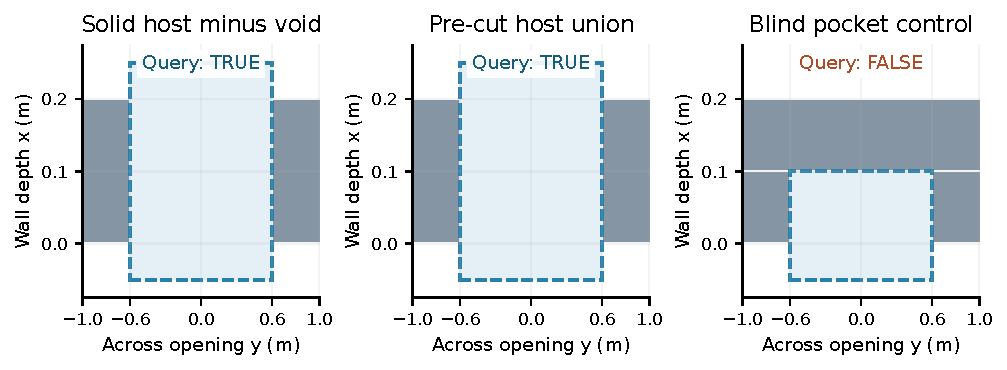
\includegraphics[width=\linewidth]{figures/verification/opening_encoding_equivalence.pdf}
\caption{Synthetic encoding-equivalence check at $z=1$ m. Gray is retained wall material; blue marks the declared void. The first two encodings yield the same material and connection verdict. The third is a true blind pocket and is rejected. Horizontal and vertical scales differ to expose the thin wall. These are software fixtures, not model outputs.}
\label{fig:opening-equivalence}
\end{figure}

The historical v1 study was generated under 2.2 and uniformly reassessed under 2.2.1 using the same retained raw outputs. Across its three routes, correct determinate readouts changed from 1,532/1,800 to 1,690/1,800: an increase of 158 measured readouts. This is a measurement correction, not improved model inference. Original outputs, original scores, and both evaluator versions remain preserved. The later N2 and CS1 cohorts prospectively use 2.2.1. The scorer checks input and evaluator freezes and compares raw-response hashes rather than selecting only favorable rescored cases.

\subsection{A remaining slab-encoding limitation}
The wall correction is not a proof of invariance for every host type. A later diagnostic examined ten preselected worlds whose issue sets were dominated by slab-opening handling. All ten transformations were attempted once. Eight preserved the occupied material and demonstrated label-sensitive geometric verdicts across ten slab-opening pairs. Two transformations changed the occupied material, so they do not establish an encoding false positive.

In the eight material-equivalent cases, the all-declared status changed from violation to unevaluable, not to pass: other unresolved checks remained. Fixed query readouts and registered statuses were unchanged in all ten attempts. The diagnostic produced no A/B all-declared pass gain and no new primary evaluator version. We therefore retain 2.2.1 primary scores and report this limitation instead of selectively substituting a more favorable encoding. The result also explains why a remaining violation count cannot automatically be read as the number of physically impossible buildings.

\subsection{Grounding, provenance, and what is not checked}
The source audit verifies whether the output names allowed sources, retains invalid active-source claims, and references existing declared entities. Given-point grounding uses exact source IDs and observation boxes, with an IoU threshold of 0.25 against approximate reference boxes. This is not camera-calibrated three-dimensional reconstruction, and source aliases are not silently normalized. A provenance edge is an inspectable declared dependency; it is not proof that a visual claim follows from its pixels. Evidence-revision experiments therefore score explicit knowledge, source status, dependencies, and retained readouts separately.

The implementation provides bounded constructive tests over rectilinear material and supported interfaces. It does not solve arbitrary three-dimensional satisfiability, certify load-bearing safety, enforce building codes, handle general meshes, or test a full human trajectory. Unknowns preserve these boundaries without counting as positive geometric success. These limits are part of the measured interface: the study tests whether models can construct and revise worlds inside that interface, while keeping answer correctness, material coherence, and visual grounding distinct.
